% Volume III, Chapter 6 -- addendum: the 2-part of the Hecke Jacobian along the canonical tower
% (open problem (b) of Section~\ref{V3P6:sec:retro}).  Verified by code/v3p6_v2_growth.py.
\section{The $2$-part along the canonical tower}\label{V3P6:sec:twopart}

This section takes up Remark~\ref{V3P6:rem:twopart}. We write $G_m=P/P_m$, $n_m=3|G_m|$,
$N_m=P_m/P_{m+1}$ and $d_m=\log_2|N_m|$, so $d_m=2$ if $3\mid m$ and $d_m=3$ otherwise
(Theorem~\ref{V3P6:thm:tower}(ii)). The vertices of $Y_m$ are the pairs $(g,s)$, $g\in G_m$,
$s\in\Z/3$, and the type-increasing arcs are $(g,s)\to(g\theta_{s,x},s+1)$, $x\in\Z/7$, with
the Schreier generators $\theta_{s,x}=\rho(a_0^{s}a_xa_0^{-(s+1)})$ of the proof of
Theorem~\ref{V3P6:thm:tower}. The group $N_m$ is central in $G_{m+1}$ and elementary abelian
(the commutator and square formulas in that proof land in $P_{m+1}$ and $P_{2m}$), and
$Y_{m+1}\to Y_m$ is a regular cover with group $N_m$. Since $\coker\DeltaH(Y_m)=\Z\oplus\JacH(Y_m)$,
the Smith form of $\DeltaH(Y_m)$ has one zero invariant factor; let $e_m$ be the number of its
\emph{even} nonzero invariant factors, i.e.\ the number of cyclic factors of even order in the
invariant-factor decomposition of $\JacH(Y_m)$, and let $\kappa_m$ be the largest $2$-adic
valuation of an invariant factor. Trivially $e_m\le v_2|\JacH(Y_m)|\le\kappa_me_m$.

\begin{proposition}[Block decomposition of a layer]\label{V3P6:prop:layer}
Fix $m\ge1$ and representatives $\tilde g\in G_{m+1}$ of the cosets of $N_m$. Every arc
$e\colon v\to w$ of $Y_m$, $v=(\bar g,s)$ with label $x$, acquires a voltage $c_e\in N_m$ by
$\tilde g_v\theta_{s,x}=c_e\tilde g_w$. For a character $\chi$ of $N_m$ (all of them are real,
with values $\pm1$) put $A_\chi=\sum_e\chi(c_e)E_{vw}$ and
$D_\chi=7I+A_\chi-2A_\chi^{t}\in M_{n_m}(\Z)$.
\begin{enumerate}
\item[(i)] $D_1=\DeltaH(Y_m)$ and $D_\chi\equiv\DeltaH(Y_m)\pmod2$ for every $\chi$. With
$H=(\chi(c))_{\chi,c}$, which satisfies $HH^{t}=2^{d_m}I$,
\[
(H\otimes I)\,\DeltaH(Y_{m+1})\,(H\otimes I)^{-1}=\bigoplus_{\chi}D_\chi .
\]
The conjugation is defined over $\Z[\tfrac12]$, not over $\Z_2$.
\item[(ii)] $\det D_\chi\ne0$ for $\chi\ne1$, and
\begin{gather*}
|\JacH(Y_{m+1})|=2^{-d_m}\,|\JacH(Y_m)|\prod_{\chi\ne1}|\det D_\chi|,\\
v_2|\JacH(Y_{m+1})|=v_2|\JacH(Y_m)|-d_m+\sum_{\chi\ne1}v_2\det D_\chi .
\end{gather*}
\item[(iii)] Each $D_\chi$, $\chi\ne1$, has exactly $e_m+1$ even invariant factors. Hence
$\sum_{\chi\ne1}v_2\det D_\chi\ge(2^{d_m}-1)(e_m+1)$ and
\[
v_2|\JacH(Y_{m+1})|\ \ge\ v_2|\JacH(Y_m)|-d_m+(2^{d_m}-1)(e_m+1).
\]
\item[(iv)] The maps $a_x\mapsto a_{2x}$ and $a_x\mapsto a_{x+1}$ are automorphisms of $\Gamma$
which extend to the tower. They act on $N_m=\{1+c\varphi^{m}\}$ by $c\mapsto c^{2}$ and
$c\mapsto\alpha^{2^{m}-1}c$, and they permute the nontrivial characters of $N_m$ transitively.
Consequently all $D_\chi$, $\chi\ne1$, have the same invariant factors over $\Z_2$.
\end{enumerate}
\end{proposition}

\begin{proof}
The lifts of $v=(\bar g,s)$ are $(c\tilde g_v,s)$, $c\in N_m$, and since $N_m$ is central the
arc of label $x$ at $c\tilde g_v$ ends at $c\tilde g_v\theta_{s,x}=c\,c_e\tilde g_w$. In the basis
indexed by $(c,v)$, $A_1(Y_{m+1})=\sum_eR(c_e)\otimes E_{vw}$, with $R$ the regular
representation of $N_m$. The characters diagonalize all $R(c)$ at once,
$HR(c)H^{-1}=\operatorname{diag}(\chi(c))$; $H\otimes I$ is real, its inverse is
$2^{-d_m}(H^{t}\otimes I)$, and transposition commutes with this conjugation. This gives the
decomposition of $\DeltaH=7+A_1-2A_1^{t}$, and $D_1=\DeltaH(Y_m)$ because the voltages of the
trivial character are $1$. Between two vertices of $Y_m$ there is at most one arc, so $A_\chi$
has entries $\pm1$ exactly on the arcs, and $D_\chi\equiv\DeltaH(Y_m)$ modulo $2$. Finally
$\det H=\pm2^{d_m2^{d_m-1}}$, so $H$ is not invertible over $\Z_2$. This proves (i).

(ii) The spectrum of $\DeltaH(Y_{m+1})$ is the union of the spectra of the $D_\chi$. Its kernel
is $\C\mathbf 1$ by the sector lemma (Lemma~\ref{V3P1:lem:sector}), and it lies in the trivial
block, so the $D_\chi$, $\chi\ne1$, are nonsingular. The product of the nonzero eigenvalues of
$\DeltaH(Y)$ is $\pm n_Y|\JacH(Y)|$ (proof of Theorem~\ref{V3P1:thm:deriv}; this is the step
used in Theorem~\ref{V3P6:thm:main}(iv)). Dividing the identities for $Y_{m+1}$ and $Y_m$, with
$n_{m+1}/n_m=2^{d_m}$, gives the product formula, and $v_2$ of it gives the valuation identity.
This is the class number formula of Theorem~\ref{V3P6:thm:main}(iv) for the layer
$Y_{m+1}/Y_m$, where it is unconditional (Remark~\ref{V3P6:rem:check}).

(iii) For a nonsingular integer matrix, the number of even invariant factors is its corank over
$\F_2$. By (i) the $\F_2$-corank of $D_\chi$ equals that of $\DeltaH(Y_m)$, which is $e_m+1$
because of the zero invariant factor. Each even invariant factor contributes at least $1$ to
$v_2\det D_\chi$, and there are $2^{d_m}-1$ nontrivial characters.

(iv) The set $T$ is invariant under $x\mapsto2x$ and $x\mapsto x+1$ (line (SY)), so both maps
are automorphisms of $\Gamma$, and they preserve $\Gamma^{0}$. On $D$ the first is induced by the
Frobenius $\sigma$ applied to the coefficients of $\F_8[[\varphi;\sigma]]$, which is a ring
automorphism because $\sigma$ commutes with itself; the second by conjugation with $\alpha^{-1}$,
since $\alpha^{-1}(\alpha^{x}\varphi)\alpha=\alpha^{x-1}\sigma(\alpha)\varphi=\alpha^{x+1}\varphi$.
Both fix the centre and the filtration $1+\varphi^{m}\mathcal O$, so they preserve every
$U_m=\Gamma^{0}\cap\rho^{-1}(P_m)$ and induce type-preserving automorphisms $\psi_m$ of the
$Y_m$ that commute with the projections (checked on the vertex model for $m\le5$ in line (SY)). On
$N_m$: $\sigma(1+c\varphi^{m})=1+c^{2}\varphi^{m}$ and
$\alpha^{-1}(1+c\varphi^{m})\alpha=1+\alpha^{-1}c\,\sigma^{m}(\alpha)\varphi^{m}
=1+\alpha^{2^{m}-1}c\,\varphi^{m}$. If $3\nmid m$, then $2^{m}\not\equiv1\pmod7$, so
$\alpha^{2^{m}-1}$ generates $\F_8^{\times}$, and multiplication by it is transitive on the
nontrivial characters of $\F_8$ (identified with $\F_8^{\times}$ through the trace form). If
$3\mid m$, then $N_m=\F_8/\F_2$, on which $\sigma$ has order $3$ and no nonzero fixed point, so
it permutes the three nontrivial characters cyclically. Now let $\psi$ be one of these
automorphisms of the layer, with $\psi(c\cdot\tilde y)=f(c)\cdot\psi(\tilde y)$ for $c\in N_m$.
Writing $\psi(\tilde g_v)=b_v\tilde g_{\psi v}$ with $b_v\in N_m$, the voltage of the image arc is
$c_{\psi e}=f(c_e)\,b_wb_v^{-1}$. Hence $A_\chi$, after the vertex permutation $\psi$, equals
$B\,A_{\chi\circ f}\,B^{-1}$ with $B=\operatorname{diag}(\chi(b_v))$: the blocks of $\chi$ and
$\chi\circ f$ are conjugate by a signed permutation matrix, which is unimodular, and they have
the same Smith form. The orbits of $f$ on the nontrivial characters are transitive, which proves
(iv). The common valuations are $12$, $64$ and $208$ for the layers $m=2,3,4$ (line (V2)).
\end{proof}

\begin{theorem}[The $2$-part at level $5$]\label{V3P6:thm:v2five}
$v_2|\JacH(Y_5)|=1742$, with $n_5=6144$. The invariant factors of $\DeltaH(Y_5)$ have the
$2$-adic profile of Table~\ref{V3P6:tab:twopart}, with $e_5=546$ even factors and
$\kappa_5=11$.
\end{theorem}

\begin{proof}
Proposition~\ref{V3P6:prop:layer}(ii) for the layer $Y_5\to Y_4$ ($d_4=3$, seven twisted blocks
of size $768$) gives $v_2|\JacH(Y_5)|=289-3+7\cdot208=1742$. The valuations $v_2\det D_\chi$
are computed by $2$-adic elimination modulo $2^{30}$, which never reaches the cap (every block
ends with no zero invariant factor, and $\DeltaH(Y_m)$ with exactly one). The same procedure
recovers $99=18-3+7\cdot12$ for $Y_3\to Y_2$ and $289=99-2+3\cdot64$ for $Y_4\to Y_3$ from the
values of Remark~\ref{V3P6:rem:twopart}, which are themselves obtained by direct elimination
(line (V2)); the exact Smith forms at levels $2$ and $3$ agree with the eliminations (line (SM)),
and the traces $\Tr A_1(Y_{m+1})^{k}$, $k=3,6$, equal the sums of the block traces (line (BL)).
Independently, the direct $2$-adic elimination of the $6144\times6144$ matrix gives $1742$
again, together with the profile of the table (line (FD), about three minutes). The block
decomposition also gives $\frac1{n_5}\log|\JacH(Y_5)|=2.062520$, the value of
Theorem~\ref{V3P6:thm:growth} that was obtained there from the full spectrum (line (TO)).
\end{proof}

The number $e_m$ is an invariant of the group ring $\F_2[G_m]$.

\begin{proposition}[Even invariant factors and the Schur complement]\label{V3P6:prop:schur}
Let $\bar f_s=\sum_{x}\theta_{s,x}^{-1}\in\F_2[G_m]$ and $F_m=1+\bar f_1\bar f_0\bar f_2$, and
let $C_m=\F_2[G_m]/\F_2[G_m]F_m$.
\begin{enumerate}
\item[(i)] $\ker_{\F_2}\bigl(\DeltaH(Y_m)\bmod2\bigr)=\ker(I+A_1)\cong\{v\in\F_2[G_m]:vF_m=0\}$,
and $e_m+1=\dim_{\F_2}C_m$.
\item[(ii)] $F_m$ lies in the augmentation ideal $I$ of $\F_2[G_m]$, the projection
$\F_2[G_{m+1}]\to\F_2[G_m]$ maps $F_{m+1}$ to $F_m$, and
$C_{m+1}/I_{N_m}C_{m+1}\cong C_m$, where $I_{N_m}$ is the augmentation ideal of $\F_2[N_m]$.
\item[(iii)] $e_{m+1}\ge e_m$, and $(e_{m+1}+1)/n_{m+1}\le(e_m+1)/n_m$. Hence the limit
$c_e=\lim_m(e_m+1)/n_m$ exists.
\item[(iv)] For $m=2,\dots,5$: $e_m=6,36,99,546$, $\dim C_m=7,37,100,547$, and
$F_m\in I^{3}\setminus I^{4}$ (the Loewy lengths of $\F_2[G_m]$ are $4,10,16,28$). The resulting
bound $e_m+1\ge\dim\F_2[G_m]/I^{3}=10$ ($m\ge3$) does not grow with $m$.
\end{enumerate}
\end{proposition}

\begin{proof}
(i) Identify $\F_2^{V(Y_m)}=\bigoplus_{s}\F_2[G_m]$ by $v\mapsto(v_s)_s$,
$v_s=\sum_gv(g,s)\,g$. Then $(A_1v)(g,s)=\sum_xv(g\theta_{s,x},s+1)$, i.e.\ $(A_1v)_s=v_{s+1}\bar f_s$
(right multiplication, which commutes with the left action of $G_m$). In characteristic $2$,
$v\in\ker(I+A_1)$ iff $v_s=v_{s+1}\bar f_s$ for all $s$, i.e.\ $v_1=v_2\bar f_1$,
$v_0=v_2\bar f_1\bar f_0$ and $v_2=v_0\bar f_2=v_2\bar f_1\bar f_0\bar f_2$. So $v$ is determined
by $v_2$, and $v_2$ is admissible iff $v_2F_m=0$. The left annihilator of $F_m$ is the kernel of
the right multiplication $R_{F_m}$ on $\F_2[G_m]$, whose dimension equals $\dim\coker R_{F_m}
=\dim C_m$. Finally $\dim\ker_{\F_2}\DeltaH(Y_m)$ is the number of invariant factors divisible
by $2$, which is $e_m+1$ (line (E) computes both sides).

(ii) The augmentation of $F_m$ is $1+7^{3}=344\equiv0$. The projection is a ring map sending
$\theta_{s,x}$ to $\theta_{s,x}$, with kernel $I_{N_m}\F_2[G_{m+1}]$ (a two-sided ideal, $N_m$
being normal). $C_{m+1}$ is a left $\F_2[G_{m+1}]$-module, since left multiplication commutes
with $R_{F_{m+1}}$, and $C_{m+1}/I_{N_m}C_{m+1}=\F_2[G_m]/\F_2[G_m]F_m=C_m$.

(iii) $C_m$ is a quotient of $C_{m+1}$, so $e_{m+1}\ge e_m$. The ring $\F_2[N_m]$ is local with
nilpotent maximal ideal $I_{N_m}$ ($N_m$ is a $2$-group). By Nakayama's lemma, lifts of a basis
of $C_m=C_{m+1}/I_{N_m}C_{m+1}$ generate $C_{m+1}$ over $\F_2[N_m]$, so
$\dim C_{m+1}\le|N_m|\dim C_m$, i.e.\ $(e_{m+1}+1)/n_{m+1}\le(e_m+1)/n_m$. A non-increasing
sequence of nonnegative numbers converges.

(iv) Lines (E) and (AU): $I^{k}$ is computed as $\sum_gI^{k-1}(g-1)$ over three generators of
$G_m$, and $F_m$ is reduced against a basis of $I^{k}$. Since the projections map $I^{k}$ onto
$I^{k}$, the depth of $F_m$ is non-increasing in $m$, so $F_m\notin I^{4}$ for all $m\ge2$.
\end{proof}

\begin{theorem}[Bounds]\label{V3P6:thm:v2bounds}
For $m\ge2$:
\begin{enumerate}
\item[(i)] $e_m\le v_2|\JacH(Y_m)|\le\kappa_me_m$, and
$v_2|\JacH(Y_m)|\le\log_2|\JacH(Y_m)|=(h_H(2)/\log2+o(1))\,n_m$ with $h_H(2)/\log2=2.977$.
\item[(ii)] $\dfrac{v_2|\JacH(Y_{m+1})|}{n_{m+1}}\ \ge\ (1-2^{-d_m})\,\dfrac{e_m+1}{n_m}\ \ge\
\tfrac34\,c_e$.
\item[(iii)] If $c_e>0$, then $v_2|\JacH(Y_m)|$ grows linearly in $n_m$:
\[
\liminf_{m\to\infty}\frac{v_2|\JacH(Y_m)|}{n_m}\ \ge\ \tfrac34\,c_e .
\]
If $v_2|\JacH(Y_m)|=o(n_m)$, then $c_e=0$, that is, $e_m=o(n_m)$. If moreover
$\kappa_m=O(\log n_m)$, then $c_e=0$ implies $v_2|\JacH(Y_m)|=o(n_m\log n_m)$.
\end{enumerate}
\end{theorem}

\begin{proof}
(i) is the definition of $e_m$ and $\kappa_m$, and Theorem~\ref{V3P6:thm:growth}.
(ii) By Proposition~\ref{V3P6:prop:layer}(iii),
$v_2|\JacH(Y_{m+1})|\ge v_2|\JacH(Y_m)|-d_m+(2^{d_m}-1)(e_m+1)$, and
$v_2|\JacH(Y_m)|\ge e_m\ge e_2=6\ge d_m$ by Proposition~\ref{V3P6:prop:schur}(iii). Since
$2^{d_m}-1=(n_{m+1}-n_m)/n_m$, dividing by $n_{m+1}$ gives the first inequality, and
$(e_m+1)/n_m\ge c_e$ for every $m$ gives the second. (iii) follows from (i) and (ii).
\end{proof}

\begin{table}[ht]
\centering\small
\renewcommand{\arraystretch}{1.15}
\resizebox{\textwidth}{!}{%
\begin{tabular}{rrrrcccl}
\toprule
$m$ & $n_m$ & $v_2|\JacH(Y_m)|$ & $e_m$ & $v_2/n_m$ & $e_m/n_m$ & $\kappa_m$ & $2$-adic profile of the invariant factors\\
\midrule
1 & 3 & 0 & 0 & 0 & 0 & 0 & --- ($|\JacH(X_3)|=147$)\\
2 & 24 & 18 & 6 & 0.7500 & 0.2500 & 3 & $2^{3}\colon6$\\
3 & 192 & 99 & 36 & 0.5156 & 0.1875 & 6 & $2^{1}\colon9,\ 2^{2}\colon9,\ 2^{3}\colon12,\ 2^{6}\colon6$\\
4 & 768 & 289 & 99 & 0.3763 & 0.1289 & 8 & $2^{1}\colon24,\ 2^{2}\colon23,\ 2^{3}\colon25,\ 2^{4}\colon9,\ 2^{5}\colon12,\ 2^{8}\colon6$\\
5 & 6144 & 1742 & 546 & 0.2835 & 0.0889 & 11 & $2^{1}\colon132,\ 2^{2}\colon83,\ 2^{3}\colon111,\ 2^{4}\colon104,\ 2^{5}\colon64,$\\
  &      &      &     &        &        &    & $2^{6}\colon25,\ 2^{7}\colon9,\ 2^{8}\colon12,\ 2^{11}\colon6$\\
\bottomrule
\end{tabular}}
\caption{The $2$-part of the Hecke Jacobian along the canonical tower. ``$2^{k}\colon c$'' means
$c$ invariant factors of $2$-adic valuation exactly $k$. Lines (SM), (V2), (E), (FD), (TB) of
\texttt{code/v3p6\_v2\_growth.py}.}\label{V3P6:tab:twopart}
\end{table}

\begin{remark}[The data, and what they support]\label{V3P6:rem:v2verdict}
Table~\ref{V3P6:tab:twopart} and line (GR) give the following.
\begin{enumerate}
\item[(a)] $v_2/n_m=0.7500$, $0.5156$, $0.3763$, $0.2835$ for $m=2,\dots,5$, decreasing at
every level. The ratios $v_2(m)/v_2(m-1)$ are $5.500$, $2.919$, $6.028$ against the indices
$8$, $4$, $8$, i.e.\ the local exponents $\log(v_2\text{ ratio})/\log(\text{index})$ are
$0.820$, $0.773$, $0.864$, and the least-squares fit $v_2\sim cn^{\beta}$ over $m=2,\dots,5$
gives $\beta=0.822$ ($0.830$ over $m=3,\dots,5$). Per unit of index, $v_2/(n_m/3)=2.250$,
$1.547$, $1.129$, $0.851$.
\item[(b)] $(e_m+1)/n_m=0.2917$, $0.1927$, $0.1302$, $0.0890$, non-increasing as
Proposition~\ref{V3P6:prop:schur}(iii) requires, with successive ratios $0.661$, $0.676$,
$0.684$. The lower bound of Theorem~\ref{V3P6:thm:v2bounds}(ii) is $0.2552$, $0.1445$, $0.1139$
at $m=3,4,5$, against the actual $0.5156$, $0.3763$, $0.2835$; the layer sums
$\sum_{\chi\ne1}v_2\det D_\chi=84$, $192$, $1456$ exceed the bounds $(2^{d_m}-1)(e_m+1)=49$,
$111$, $700$ by the factors $1.71$, $1.73$, $2.08$.
\item[(c)] At every computed level the largest exponent is $\kappa_m=\log_2|G_m|=\log_2(n_m/3)$
($3,6,8,11$), attained by exactly six invariant factors: the $2$-part of $\JacH(Y_m)$ has
exponent $|G_m|$ and contains $(\Z/|G_m|)^{6}$. We have no explanation. The invariant factors of
the twisted blocks (largest exponent $5$ at the layer $Y_5\to Y_4$) are not those of
$\DeltaH(Y_5)$, as Proposition~\ref{V3P6:prop:layer}(i) warns.
\end{enumerate}
\emph{Verdict.} The conjecture that $\lim v_2|\JacH(Y_m)|/n_m$ exists and is positive is
\emph{not supported by the data}: on the five computed levels the ratio decreases monotonically
from $0.75$ to $0.28$, every local exponent is below $1$, and $(e_m+1)/n_m$ decays geometrically
by a factor of about $0.68$ per level. The data support \emph{sublinear} growth,
$v_2|\JacH(Y_m)|\asymp n_m^{\beta}$ with $\beta\approx0.82$, and, through
Theorem~\ref{V3P6:thm:v2bounds}(iii), they suggest $c_e=0$. This is a statement about five
levels only; the levels $6$--$8$ of Theorem~\ref{V3P6:thm:v2eight} and
Remark~\ref{V3P6:rem:v2eight} weaken it (the decay rates are slowing down), and
Theorem~\ref{V3P6:thm:v2sharp} improves the constant $\frac34$ below to $1$. We have no proof of an asymptotic law in either direction. What is proved is
Theorem~\ref{V3P6:thm:v2bounds}: linear growth follows from $c_e>0$, sublinear growth forces
$c_e=0$, and $c_e$ is the limit of the normalized kernel dimensions of the single element $F_m$
of $\F_2[G_m]$, a mod-$2$ analogue of a von Neumann dimension along the tower, whose
vanishing is the real open question. The augmentation filtration does not decide it: $F_m$ has
depth exactly $3$ for all computed $m$, which gives only $e_m+1\ge10$. Because $P$ has infinite
rank (Theorem~\ref{V3P6:thm:tower}(iii)), $\F_2[[P]]$ is not known to be Noetherian, and the
growth bounds for torsion modules over the Iwasawa algebras of $p$-adic analytic groups are not
available. Open problem (b) of Section~\ref{V3P6:sec:retro} is therefore sharpened to: decide
whether
\[
c_e=\lim_{m\to\infty}\frac{\dim_{\F_2}\bigl(\F_2[G_m]/\F_2[G_m]F_m\bigr)}{n_m}
\]
vanishes.
\end{remark}

\subsection*{Induced characters and levels $6$--$8$}

The layer decomposition of Proposition~\ref{V3P6:prop:layer} uses the central subgroup $N_m$, so
each new level costs $2^{d_m}-1$ blocks of the size of the previous level. Going down to
$Y_k$ with $k\approx m/2$ is much cheaper, because the whole kernel $P_k/P_m$ is still abelian.

\begin{proposition}[Induced characters of $P_k/P_m$]\label{V3P6:prop:induced}
Let $2\le k<m\le2k$ and $A=P_k/P_m\subset G_m$.
\begin{enumerate}
\item[(i)] $A$ is an elementary abelian normal $2$-subgroup, and the coefficients of
$\varphi^{k},\dots,\varphi^{m-1}$ (without the $\F_2$-part of the coefficients of $\varphi^{3i}$)
identify it with $\F_2^{d}$, $2^{d}=n_m/n_k$. The left action of $A$ on $Y_m$ is free, and
$A\backslash Y_m=Y_k$.
\item[(ii)] With coset representatives $r_c\in G_m$ ($c\in G_k$), every arc $c\to c'$ of $Y_k$ with
label $x$ has the voltage $a_e=r_c\theta_{s,x}r_{c'}^{-1}\in A$. For $\chi\in\widehat A$ put
$A_\chi=\sum_e\chi(a_e)E_{cc'}$ and $D_\chi=7I+A_\chi-2A_\chi^{t}$. Then
$\DeltaH(Y_m)$ is conjugate over $\Z[\frac12]$ to $\bigoplus_\chi D_\chi$, $D_1=\DeltaH(Y_k)$,
$D_\chi\equiv\DeltaH(Y_k)\pmod2$, and
\[
v_2|\JacH(Y_m)|=v_2|\JacH(Y_k)|-\log_2\frac{n_m}{n_k}+\sum_{\chi\ne1}v_2\det D_\chi .
\]
\item[(iii)] (Artin--Clifford.) $D_\chi$ is the Hecke operator of $Y_k$ twisted by
$\operatorname{Ind}_A^{G_m}\chi$. $G_m$ acts on $\widehat A$ by conjugation; blocks in one orbit
$O$ are conjugate by signed permutation matrices, hence have the same Smith form over $\Z_2$, and
\[
\prod_{\chi\in O}\det D_\chi=\prod_{\rho\in\operatorname{Irr}(G_m)\text{ over }O}\det\bigl(\Delta^{H}_\rho\bigr)^{\dim\rho}.
\]
\end{enumerate}
\end{proposition}

\begin{proof}
(i) $A$ is the kernel of the projection $G_m\to G_k$, hence normal. For $x,y\in\varphi^{k}\mathcal O$,
$(1+x)(1+y)=1+x+y+xy$ and $xy\in\varphi^{2k}\mathcal O\subseteq\varphi^{m}\mathcal O$, so $A$ is
abelian, the multiplication is addition of coefficients, and every element has order $2$. The
central units $1+t^{i}$ used to normalize only change the $\F_2$-part of the coefficient of
$\varphi^{3i}$, and they also act additively, since the cross terms again lie in
$\varphi^{2k}\mathcal O$. The deck group $G_m$ acts on $Y_m$ by left multiplication and the arcs
are right multiplications, so the left action of any subgroup is free and commutes with the arcs.
(ii) The arc of label $x$ at $ar_c$ ends at $ar_c\theta_{s,x}=(aa_e)r_{c'}$. In the basis
$(a,c)$, $A_1(Y_m)=\sum_eR(a_e)\otimes E_{cc'}$, and the proof of
Proposition~\ref{V3P6:prop:layer}(i)--(ii) applies word for word with $A$ in place of $N_m$; it
never used that $N_m$ is central, only that it is abelian and acts on the left. (iii)
$\C[G_m]=\operatorname{Ind}_A^{G_m}\C[A]=\bigoplus_\chi\operatorname{Ind}_A^{G_m}\chi$, and the
$\chi$-summand is the $\chi$-isotypic part for the left $A$-action, on which $\DeltaH$ acts as
$D_\chi$. For $g\in G_m$, left multiplication by $g$ maps $ar_c$ to $(gag^{-1})(gr_c)$ and
$gr_c=b_cr_{\bar gc}$ with $b_c\in A$; it carries the $\chi$-isotypic part to the
$\chi\circ\operatorname{Ad}(g)^{-1}$-isotypic part, and in the bases above it is the
permutation $c\mapsto\bar gc$ times the signs $\chi(b_c)$. By Clifford's theorem every
irreducible $\rho$ of $G_m$ lies over exactly one orbit, and
$\bigoplus_{\chi\in O}\operatorname{Ind}\chi=\bigoplus_{\rho\text{ over }O}\rho^{\dim\rho}$ as
summands of the regular representation; take determinants of $\DeltaH$ on both sides.
\end{proof}

\begin{theorem}[Levels $6$, $7$, $8$]\label{V3P6:thm:v2eight}
The $2$-parts and the total orders of the Hecke Jacobians of $Y_5,\dots,Y_8$ are:
\begin{center}\small
\begin{tabular}{rrrcc}
\toprule
$m$ & $n_m$ & $v_2|\JacH(Y_m)|$ & $v_2/n_m$ & $\frac1{n_m}\log|\JacH(Y_m)|$\\
\midrule
$5$ & $6144$ & $1742$ & $0.28353$ & $2.062520$\\
$6$ & $49152$ & $11595$ & $0.23590$ & $2.063511$\\
$7$ & $196608$ & $36937$ & $0.18787$ & $2.063639$\\
$8$ & $1572864$ & $254662$ & $0.16191$ & $2.063684$\\
\bottomrule
\end{tabular}
\end{center}
\end{theorem}

\begin{proof}
Proposition~\ref{V3P6:prop:induced} with $(m,k)=(6,3)$: $255$ blocks of size $192$ in $24$
conjugation orbits; $(6,4)$: $63$ blocks of size $768$ in $21$ orbits; $(7,4)$: $255$ blocks in $24$
orbits; $(8,4)$: $2047$ blocks of size $768$ in $52$ orbits (sizes $1^{7},4^{14},64^{31}$). The
block valuations are computed by the $2$-adic elimination of Theorem~\ref{V3P6:thm:v2five} (cap
$2^{30}$, never reached), on one representative of each orbit, and checked to be constant on the
orbit (all members for $m\le6$, two further members of every orbit for $m=7,8$). The two routes to
level $6$ give $99+7-15+11504=289+9-15+11312=11595$, and the two routes to level $7$, over
$Y_4$ and over $Y_5$ ($(m,k)=(7,5)$: $31$ blocks of size $6144$ in $10$ orbits, valuations $1408$
and $1056$), give $289+9-17+36656=1742+12-17+35200=36937$. The same procedure recovers $99$, $289$
and $1742$ from $Y_2$ and $Y_3$, i.e.\ Theorem~\ref{V3P6:thm:v2five} by a route independent of the
central layers. The total orders are the sums of $\log|\det D_\chi|$ (floating point).
\end{proof}

The column of total orders converges to $h_H=2.063693$ from below, the last value being
$9\cdot10^{-6}$ short: the Plancherel limit of Theorem~\ref{V3P6:thm:growth} is visible to five
digits at $n=1.57\cdot10^{6}$. The $2$-part does not converge at that rate, if at all.

\begin{theorem}[A sharper lower bound]\label{V3P6:thm:v2sharp}
For $2\le k<m\le2k$,
\[
v_2|\JacH(Y_m)|\ \ge\ v_2|\JacH(Y_k)|-\log_2\frac{n_m}{n_k}+\Bigl(\frac{n_m}{n_k}-1\Bigr)(e_k+1).
\]
Consequently $\liminf_m v_2|\JacH(Y_m)|/n_m\ge c_e$, improving the constant $\frac34$ of
Theorem~\ref{V3P6:thm:v2bounds}(iii) to $1$. Moreover $e_6=3169$, so
$c_e\le(e_6+1)/n_6=0.06449$.
\end{theorem}

\begin{proof}
By Proposition~\ref{V3P6:prop:induced}(ii) each of the $n_m/n_k-1$ nontrivial blocks is congruent
to $\DeltaH(Y_k)$ modulo $2$, hence has $\F_2$-corank $e_k+1$ and $v_2\det D_\chi\ge e_k+1$ (as in
Proposition~\ref{V3P6:prop:layer}(iii)). For the limit take $k=\lceil m/2\rceil$: then
$n_m/n_k\to\infty$, $\log_2(n_m/n_k)=O(m)=o(n_m)$, $v_2|\JacH(Y_k)|\ge0$, and
$(e_k+1)/n_k\ge c_e$ by Proposition~\ref{V3P6:prop:schur}(iii). The value of $e_6$ is
$\dim\F_2[G_6]/\F_2[G_6]F_6-1$ by Proposition~\ref{V3P6:prop:schur}(i), computed by Gaussian
elimination over $\F_2$ on the $16384\times16384$ matrix of right multiplication by $F_6$
($|\operatorname{supp}F_6|=154$).
\end{proof}

\begin{figure}[t]
\centering
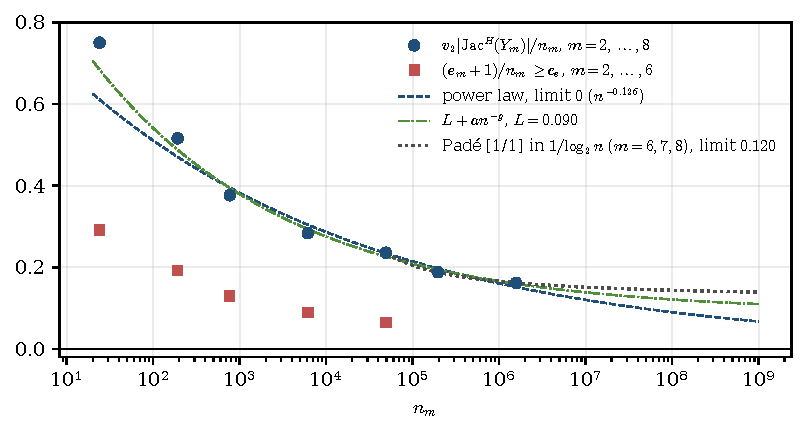
\includegraphics[width=\textwidth]{figures/fig_v2_growth.pdf}
\caption{The $2$-part of the Hecke Jacobian along the canonical $2$-tower: $v_2|\JacH(Y_m)|/n_m$ for
$m=2,\dots,8$ (Theorems~\ref{V3P6:thm:v2five}, \ref{V3P6:thm:v2eight}) and the normalized
$\F_2$-kernel dimensions $(e_m+1)/n_m$ for $m=2,\dots,6$, which decrease to the limit $c_e$
(Proposition~\ref{V3P6:prop:schur}, Theorem~\ref{V3P6:thm:v2sharp}). Three extrapolations of
$v_2/n_m$ that fit the data about equally well: a power law $n^{-0.126}$ with limit $0$ (fitted on
$m=3,\dots,8$); the least-squares optimum $0.090+an^{-g}$ of Remark~\ref{V3P6:rem:v2eight}(b); and the
Pad\'e approximant $[1/1]$ in $1/\log_2n$ through $m=6,7,8$, with limit $0.120$, drawn only on the range
of its data and beyond. The data do not decide between a positive limit and slow decay to $0$; what is
proved is $\liminf v_2/n_m\ge c_e$. Data of \texttt{code/v3p6\_level5\_v2.py}, drawn by
\texttt{code/make\_figures.py}.}
\label{V3P6:fig:v2growth}
\end{figure}

\begin{remark}[The data at levels $2$--$8$]\label{V3P6:rem:v2eight}
The numbers below are produced by lines (FT) and (E) of the script
\texttt{code/v3p6\_level5\_v2.py}.
\begin{enumerate}
\item[(a)] The sequences, with the local exponent
$\beta_m=\log\bigl(v_2(m)/v_2(m-1)\bigr)/\log(n_m/n_{m-1})$ and the ratio
$\rho_m=\bigl((e_m+1)/n_m\bigr)/\bigl((e_{m-1}+1)/n_{m-1}\bigr)$:
\begin{center}\small
\begin{tabular}{lccccccc}
\toprule
$m$ & $2$ & $3$ & $4$ & $5$ & $6$ & $7$ & $8$\\
\midrule
$n_m/n_{m-1}$ & --- & $8$ & $4$ & $8$ & $8$ & $4$ & $8$\\
$v_2/n_m$ & $0.750$ & $0.516$ & $0.376$ & $0.284$ & $0.236$ & $0.188$ & $0.162$\\
$\beta_m$ & --- & $0.820$ & $0.773$ & $0.864$ & $0.912$ & $0.836$ & $0.928$\\
$(e_m+1)/n_m$ & $0.292$ & $0.193$ & $0.130$ & $0.089$ & $0.064$ & & \\
$\rho_m$ & --- & $0.661$ & $0.676$ & $0.684$ & $0.724$ & & \\
\bottomrule
\end{tabular}
\end{center}
$v_2/n_m$ still decreases at every level, and every $\beta_m$ is below $1$. But the exponents are
increasing; along the layers of index $8$ they are $0.820$, $0.864$, $0.912$, $0.928$. Likewise
$(e_m+1)/n_m$ decreases with increasing ratios $\rho_m$, so the geometric decay by a constant factor
suggested by Remark~\ref{V3P6:rem:v2verdict}(b) is not borne out (Figure~\ref{V3P6:fig:v2growth}).
\item[(b)] \emph{Fits.} With limit $L=0$ the best power law is $v_2\sim n^{0.874}$. The
three-parameter model $v_2/n=L+an^{-g}$ fitted on $m=3,\dots,8$ has its least-squares optimum at
$L=0.090$, but the residual at $L=0$ is only $1.09$ times the optimum, and the leave-one-out optima
range over $[0,0.125]$. Exact fits through three consecutive levels jump with the period-$3$
pattern of the indices ($8,4,8,8,4,8$) and are not used. The data do not distinguish a positive
limit of order $0.1$ from slow decay to $0$.
\item[(c)] \emph{Rigorous interval.} $c_e\le\liminf v_2/n_m\le\limsup v_2/n_m\le h_H/\log2=2.977$,
with $0\le c_e\le0.0645$. The bound of Theorem~\ref{V3P6:thm:v2sharp} is far from sharp at finite
level: over $Y_4$ it gives $v_2/n_m\ge0.134,0.131,0.130$ for $m=6,7,8$, against the actual
$0.236,0.188,0.162$.
\item[(d)] \emph{The ratio to $c_e$.} At $m=2k$ the observed quotient
$\bigl(v_2|\JacH(Y_{2k})|/n_{2k}\bigr)\big/\bigl((e_k+1)/n_k\bigr)$ is $1.290,1.224,1.243$ for
$k=2,3,4$: on average a twisted block has about $1.25$ times the minimal valuation $e_k+1$. If this
quotient stays bounded, which would follow from a uniform bound on the $2$-exponents of the blocks
(they are at most $10$ at levels $6$--$8$), then $v_2|\JacH(Y_m)|/n_m$ and $(e_{\lceil m/2\rceil}+1)/n_{\lceil m/2\rceil}$ have the same
order, and $\lim v_2/n_m>0$ iff $c_e>0$.
\end{enumerate}
\emph{Verdict.} Strict positivity of the slope is not decided by levels $2$--$8$. What is proved is
that a positive mod-$2$ kernel density $c_e$ forces slope at least $c_e$; the numbers agree with
slope $\asymp c_e$, and both sequences are still decreasing, but more slowly at every level.
The open problem remains whether $c_e=\lim\dim_{\F_2}(\F_2[G_m]/\F_2[G_m]F_m)/n_m$ vanishes.
\end{remark}

\begin{remark}[Verification]\label{V3P6:rem:v2code}
The script \texttt{code/v3p6\_v2\_growth.py} uses numpy and the sparse module of scipy. It runs
in about five minutes (one minute with \texttt{--quick}, which skips line (FD)). It builds
levels $2$--$5$ (line (LV)), checks
the central elementary abelian layers and the voltages, the trace identities and the Hadamard
decomposition (BL), the valuation identity at the layers $2\to3$, $3\to4$ against the direct
values and its application at $4\to5$ (V2), the agreement of the $2$-adic eliminations with the
exact Smith forms at levels $2,3$ (SM), $e_m$ from the $\F_2$-rank of $I+A_1$ and from
$\dim C_m$ (E), the depth of $F_m$ (AU), the two automorphisms and their action on the
characters (SY), the total order and $v_2\le\log_2|\JacH|$ (TO), the direct elimination of the
$6144\times6144$ matrix (FD), and the table and growth statistics (TB), (GR).

The script \texttt{code/v3p6\_level5\_v2.py} (numpy, matplotlib; about three minutes, plus about
$70$ minutes with \texttt{--check7}) verifies Proposition~\ref{V3P6:prop:induced} and
Theorems~\ref{V3P6:thm:v2eight}, \ref{V3P6:thm:v2sharp}: the quotient models and the
elementary abelian structure of $P_k/P_m$ (QT), the conjugation orbits on the characters (CJ), the
re-derivation of $18,99,289$ by direct elimination and of $99,289,1742$ through induced characters
(VA), the new levels with the two routes to level $6$ (and, with \texttt{--check7}, the route to
level $7$ over $Y_5$) (NW), $e_m+1$ for $m\le6$ and the sharpened bound (E), the total orders (TO),
and the fits (FT). Data and the figure are written to \texttt{data/}.
\end{remark}
